\chapter{Test Specification}

%-----------------------------------------------------------------%
    %Test Case 1 - Uart Communication
%-----------------------------------------------------------------%
\section{TC-01 - UART Communication}

\renewcommand{\arraystretch}{1.4}

\begin{table}[h]
\centering
\begin{tabular}{|p{3cm}|p{12cm}|}
\hline
\textbf{Test Case ID} & TC-01 \\ \hline
\textbf{Description} & Testing UART Communication in Auth \\ \hline
\textbf{Prerequisites} & State Operational and ADC values are valid \\ \hline
\textbf{Test Steps} &
\begin{enumerate}
\item Execute the 10ms task
\item The constant \textit{PERCENTTOLERANCE} was set to 30 for testing
\item Check the if-condition (see code)
\item Inspect the values in Eclipse
\item Manually modify the ADC values
\item Set a breakpoint on \textit{applicationSendEvent()}
\item Verify at which values the breakpoint is triggered and validate the calculation
\end{enumerate}
\\ \hline
\textbf{Expected Result} & Breakpoint is triggered \\ \hline
\textbf{Actual Result} & Breakpoint is triggered and calculated values match the expected results \\ \hline
\textbf{Status} & \textcolor{green!60!black}{Passed} \\ \hline
\end{tabular}
\end{table}
\newpage
\subsection{Description TC-01}

\textbf{Tested Code:}

\begin{lstlisting}[style=CStyle]
gScheduler.pGetHALTick = HAL_GetTick;
gScheduler.pTask_10ms = task10ms;
gScheduler.pTask_50ms = task50ms;
gScheduler.pTask_250ms = task250ms;

int main(void)
{
    while(1)
    {
        task10ms();
        task50ms();
        task250ms();
    }
}

void task10ms()
{
    ledToggleLED(LED0);
}

void task50ms()
{
    ledToggleLED(LED1);
}

void task250ms()
{
    ledToggleLED(LED2);
}
\end{lstlisting}
\newpage
%-----------------------------------------------------------------%
    %Test Case 2 - Transition from Auth to App
%-----------------------------------------------------------------%
\section{TC-02 - Transition from Auth to App}

\renewcommand{\arraystretch}{1.4}

\begin{table}[h]
\centering
\begin{tabular}{|p{3cm}|p{12cm}|}
\hline
\textbf{Test Case ID} & TC-02 \\ \hline
\textbf{Description} & Testing the transition to the Failure state due to tolerance violation \\ \hline
\textbf{Prerequisites} & State Operational and ADC values are valid \\ \hline
\textbf{Test Steps} &
\begin{enumerate}
\item Execute the 10ms task
\item The constant \textit{PERCENTTOLERANCE} was set to 30 for testing
\item Check the if-condition (see code)
\item Inspect the values in Eclipse
\item Manually modify the ADC values
\item Set a breakpoint on \textit{applicationSendEvent()}
\item Verify at which values the breakpoint is triggered and validate the calculation
\end{enumerate}
\\ \hline
\textbf{Expected Result} & Breakpoint is triggered \\ \hline
\textbf{Actual Result} & Breakpoint is triggered and calculated values match the expected results \\ \hline
\textbf{Status} & \textcolor{green!60!black}{Passed} \\ \hline
\end{tabular}
\end{table}
\newpage
\subsection{Description TC-02}

\textbf{Tested Code:}

\begin{lstlisting}[style=CStyle]
void System_Init(void)
{
    HAL_Init();
    GPIO_Init();
    UART_Init();
}
\end{lstlisting}

\newpage
%-----------------------------------------------------------------%
    %Test Case 3 - Scheduler Functionality
%-----------------------------------------------------------------%
\section{TC-03 - Scheduler Functionality}

\renewcommand{\arraystretch}{1.4}

\begin{table}[h]
\centering
\begin{tabular}{|p{3cm}|p{12cm}|}
\hline
\textbf{Test Case ID} & TC-03 \\ \hline
\textbf{Description} & Verification of the scheduler functionality \\ \hline
\textbf{Prerequisites} & Scheduler has been initialized \\ \hline
\textbf{Test Steps} &
\begin{enumerate}
\item Configure the three required scheduler intervals
\item Use \textit{ledToggleLED()} for the test
\item Run the \textit{main\_app}
\item Observe the LEDs
\end{enumerate}
\\ \hline
\textbf{Expected Result} & LEDs should toggle after 10, 50 and 250\,ms \\ \hline
\textbf{Actual Result} & LED1 and LED2 toggle correctly. LED0 remains permanently on because the toggle rate is too fast to observe \\ \hline
\textbf{Status} & \textcolor{green!60!black}{Passed} \\ \hline
\end{tabular}
\end{table}

\newpage
\subsection{Description TC-03}

This test case verifies the correct functionality of the implemented scheduler mechanism. 
According to the system requirements, the scheduler is responsible for executing periodic 
tasks at predefined time intervals. In this test, three different tasks with execution 
intervals of 10\,ms, 50\,ms and 250\,ms are configured.

For verification purposes, the function \textit{ledToggleLED()} is used inside each task 
in order to generate a visible output on the hardware LEDs. The scheduler receives the 
system time via \textit{HAL\_GetTick()} and triggers the assigned tasks accordingly. 
The function pointers \textit{pTask\_10ms}, \textit{pTask\_50ms}, and \textit{pTask\_250ms} 
are assigned to the corresponding task functions \textit{task10ms()}, 
\textit{task50ms()}, and \textit{task250ms()}.

During execution of the \textit{main} loop, the scheduler repeatedly calls the configured 
tasks. Each task toggles a specific LED, allowing the timing behaviour to be observed 
directly on the hardware. If the scheduler operates correctly, LED1 and LED2 should toggle 
with clearly observable intervals corresponding to 50\,ms and 250\,ms. The behaviour of 
LED0 is difficult to observe due to the high frequency of the 10\,ms task.

The successful execution of this test confirms that the scheduler correctly triggers 
periodic tasks and that the system timing mechanism works according to the specified 
requirements.
\newpage
\textbf{Tested Code:}

\begin{lstlisting}[style=CStyle]
gScheduler.pGetHALTick = HAL_GetTick;
gScheduler.pTask_10ms = task10ms;
gScheduler.pTask_50ms = task50ms;
gScheduler.pTask_250ms = task250ms;

int main(void)
{
    while(1)
    {
        task10ms();
        task50ms();
        task250ms();
    }
}

void task10ms()
{
    ledToggleLED(LED0);
}

void task50ms()
{
    ledToggleLED(LED1);
}

void task250ms()
{
    ledToggleLED(LED2);
}
\end{lstlisting}
\newpage

%-----------------------------------------------------------------%
    %Test Case 4 - Tolerance of the Filtered ADC Values
%-----------------------------------------------------------------%
\section{TC-04 - Tolerance of the Filtered ADC Values}

\renewcommand{\arraystretch}{1.4}

\begin{table}[h]
\centering
\begin{tabular}{|p{3cm}|p{12cm}|}
\hline
\textbf{Test Case ID} & TC-04 \\ \hline
\textbf{Description} & Testing the transition to the Failure state due to tolerance violation \\ \hline
\textbf{Prerequisites} & State Operational and ADC values are valid \\ \hline
\textbf{Test Steps} &
\begin{enumerate}
\item Execute the 10ms task
\item The constant \textit{PERCENTTOLERANCE} was set to 30 for testing
\item Check the if-condition (see code)
\item Inspect the values in Eclipse
\item Manually modify the ADC values
\item Set a breakpoint on \textit{applicationSendEvent()}
\item Verify at which values the breakpoint is triggered and validate the calculation
\end{enumerate}
\\ \hline
\textbf{Expected Result} & Breakpoint is triggered \\ \hline
\textbf{Actual Result} & Breakpoint is triggered and calculated values match the expected results \\ \hline
\textbf{Status} & \textcolor{green!60!black}{Passed} \\ \hline
\end{tabular}
\end{table}
\newpage
\subsection{Description TC-04}
This test case verifies the correct detection of inconsistent gas sensor values based on a defined tolerance threshold. 
The filtered values of the two gas sensors are compared within the periodic \textit{10ms task} using the function 
\textit{isGasSensorMismatch()}.

If the calculated deviation between \textit{pot1\_filtered} and \textit{pot2\_filtered} exceeds the tolerance defined by 
\textit{PERCENTTOLERANCE}, the function signals a mismatch and the application triggers the event 
\textit{APP\_EVT\_SENSOR\_DEFECT} via \textit{applicationSendEvent()}.

For testing purposes, the tolerance was increased to 30\,\% and the ADC values were manually modified in the debugger 
to generate controlled deviations. A breakpoint was placed on \textit{applicationSendEvent()} to verify that the event 
is triggered once the defined tolerance threshold is exceeded.

The successful execution of this test confirms that the system correctly detects inconsistent sensor readings and 
handles tolerance violations according to the specified requirements.

\textbf{Tested Code:}

\begin{figure}[h]
    \centering
    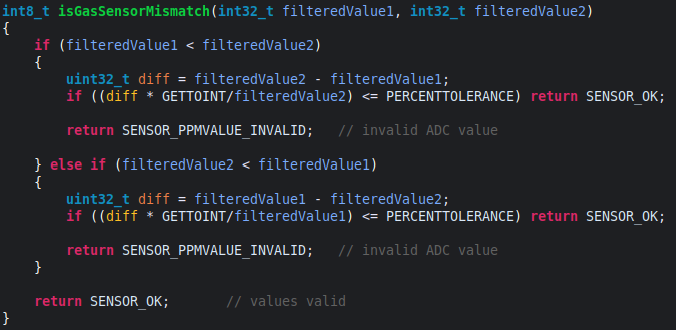
\includegraphics[width=0.85\linewidth]{Pictures/t4.png}
    \caption{Tested code for TC-04}
    \label{fig:t4_code}
\end{figure}
\newpage

%-----------------------------------------------------------------%
    %Test Case 5 - Check State Machine Transition
%-----------------------------------------------------------------%
\section{TC-05 - Check State Machine Transition}

\renewcommand{\arraystretch}{1.4}

\begin{table}[h]
\centering
\begin{tabular}{|p{3cm}|p{12cm}|}
\hline
\textbf{Test Case ID} & TC-05 \\ \hline
\textbf{Description} & Testing the transition to the Failure state from Init \\ \hline
\textbf{Prerequisites} & Start the app and sensor values are invalid \\ \hline
\textbf{Test Steps} &
\begin{enumerate}
\item Start the program
\item Force the transition to Failure by using sensor values
\item Run the scheduler
\item The 10ms task for initialization is executed (an LED was used here)
\item Let it run through 5 cycles
\end{enumerate}
\\ \hline
\textbf{Expected Result} & After the 50ms task is called, the app should be in the Failure state \\ \hline
\textbf{Actual Result} & Breakpoint is reached and the state switch works correctly \\ \hline
\textbf{Status} & \textcolor{green!60!black}{Passed} \\ \hline
\end{tabular}
\end{table}
\newpage
\subsection{Description TC-05}

This test case verifies the correct transition of the application state machine from the 
\textit{Initialization} state to the \textit{Failure} state when invalid sensor values are detected. 
During system startup, the sensor values are checked using the function 
\textit{checkForValideADC()}.

If invalid values are detected, the application triggers the event 
\textit{APP\_EVT\_ERROR} via \textit{applicationSendEvent()}, which should lead to a 
state transition into the failure handling state.

During the test, breakpoints were placed at the event trigger and within the state machine 
implementation. The scheduler executes the periodic tasks and the \textit{10ms task} initially 
runs in the \textit{APP\_STATE\_INITIALIZATION} state. After several cycles, the application 
should switch to \textit{APP\_STATE\_FAILURE}, which was verified by reaching the corresponding 
breakpoint.

The successful execution of this test confirms that the state machine correctly processes 
error events and performs the expected transition to the failure state.

\textbf{Tested Code:}

\begin{lstlisting}[style=CStyle]
if (checkForValideADC(gasSensorReadPpmValue(&gGasSensor1, ADC_INPUT0), gasSensorReadPpmValue(&gGasSensor2, ADC_INPUT1)))
        {
            applicationSendEvent(APP_EVT_ERROR); // Breakpoint here to force the error state
        }
void taskApp10ms()
{
    // (...)
    case APP_STATE_INITIALIZATION:
        // Breakpoint here should be passed for 5 cycles
        ledToggleLED(LED3); 
        break;
    case APP_STATE_FAILURE:
        // Breakpoint to be reached here
        ledToggleLED(LED4);
        break;
}
\end{lstlisting}
\newpage

%-----------------------------------------------------------------%
    %Test Case 6 - Problematic Sensor Values During Initialization
%-----------------------------------------------------------------%
\section{TC-06 - Problematic Sensor Values During Initialization}

\renewcommand{\arraystretch}{1.4}

\begin{table}[h]
\centering
\begin{tabular}{|p{3cm}|p{12cm}|}
\hline
\textbf{Test Case ID} & TC-06 \\ \hline
\textbf{Description} & Problematic sensor values during initialization \\ \hline
\textbf{Prerequisites} & Start the app \\ \hline
\textbf{Test Steps} &
\begin{enumerate}
\item Debug the system
\item Set breakpoints on the values and read them out
\item Inspect the values in Eclipse
\item Set a breakpoint on \textit{applicationSendEvent()}
\item Verify which breakpoint is hit
\end{enumerate}
\\ \hline
\textbf{Expected Result} & Breakpoint is reached and the system should transition to PreOperational state \\ \hline
\textbf{Actual Result} & The Failure breakpoint is reached. The values should only be between 200 - 10000 or -1, -2, -3 in case of errors, but invalid values occurred. By adding a short delay before reading, the first values become valid \\ \hline
\textbf{Status} & \textcolor{green!60!black}{Conditionally Passed} \\ \hline
\end{tabular}
\end{table}
\newpage
\subsection{Description TC-06}
This test case analyzes the behaviour of the system during the initialization phase when the gas sensor values are read for the first time. 
During testing it was observed that the initial ADC readings of the sensors were not yet valid immediately after initialization. 
As a result, the validation check in \textit{checkForValideADC()} incorrectly detected invalid sensor values and triggered the event 
\textit{APP\_EVT\_ERROR}, causing the application to transition into the \textit{Failure} state.

Further debugging showed that the sensors require a short stabilization time before providing valid measurements. 
If the sensor values were read a second time shortly after the first read, the values were already within the expected range. 
To ensure reliable initialization, a short delay using \textit{HAL\_Delay()} was introduced before performing the first validation check.

After adding the delay, the sensor readings became valid and the system correctly transitioned to the 
\textit{PreOperational} state instead of entering the failure state. 
This test confirms that the initialization sequence must allow sufficient time for the sensors to stabilize before validating their values.

\textbf{Tested Code:}

\begin{lstlisting}[style=CStyle]
int32_t onEntryInitialization(State_t* pState, int32_t eventID)
{
    // (...)
    gasSensorInitialize(&gGasSensor1, 204);
    gasSensorInitialize(&gGasSensor2, 204);

    HAL_Delay(30);  // Testing showed that a delay is necessary here because the sensor needs time to provide valid values. Otherwise, the app immediately switches to Failure because the ADCs do not yet provide valid values at this time.

    if (checkForValideADC(gasSensorReadPpmValue(&gGasSensor1, ADC_INPUT0), gasSensorReadPpmValue(&gGasSensor2, ADC_INPUT1)))
    {
        applicationSendEvent(APP_EVT_ERROR);
    }

    applicationSendEvent(APP_EVT_INIT_DONE);
}

int32_t gasSensorReadPpmValue(GasSensor* pSensor, ADC_Channel_t adcChannel)
{
    uint32_t raw = adcReadChannel(adcChannel);

    gasSensorSetSensorVoltage(pSensor, raw);

    return gasSensorGetSensorValue(pSensor);
}

int32_t gasSensorGetSensorValue(GasSensor* pSensor) {
	if (!pSensor) return SENSOR_INVALID_PTR;

	int32_t value = (int32_t)(pSensor->sensorVoltage / pSensor->conversionFactor);

	if (value < MIN_SENSOR_VALUE || value > MAX_SENSOR_VALUE) return SENSOR_VALUE_INVALID;

	return value;
}
\end{lstlisting}

\newpage

%-----------------------------------------------------------------%
    %Test Case 7 - Display Visualization
%-----------------------------------------------------------------%
\section{TC-07 - Display Visualization}

\renewcommand{\arraystretch}{1.4}

\begin{table}[h]
\centering
\begin{tabular}{|p{3cm}|p{12cm}|}
\hline
\textbf{Test Case ID} & TC-07 \\ \hline
\textbf{Description} & Testing the display visualization with valid values \\ \hline
\textbf{Prerequisites} & State Operational and water values are valid \\ \hline
\textbf{Test Steps} &
\begin{enumerate}
\item Manually giving texting values to the display (230, 280, 1000)
\item Let the loop run for exact values
\item Check the display and verify that the values are displayed correctly
\end{enumerate}
\\ \hline
\textbf{Expected Result} & Left and right display show correct values \\ \hline
\textbf{Actual Result} & See expected result \\ \hline
\textbf{Status} & \textcolor{green!60!black}{Passed} \\ \hline
\end{tabular}
\end{table}
\newpage
\subsection{Description TC-07}
This test case verifies the correct visualization of valid water level values on the display during the 
\textit{Operational} state. For testing purposes, fixed test values were manually provided instead of the 
original sensor input to ensure deterministic behaviour.

The values 230, 280 and 1000 were used as input to the display logic inside the function 
\textit{waterSensorHandler()}. The display is updated periodically and alternates between the left and 
right digit in order to visualize the complete value.

During testing it was observed that the value 1000 is still within the valid sensor range, but the display 
is limited by the constant \textit{MAX\_DISPLAY\_VALUE}. Therefore the maximum representable value on the 
display is shown instead of the full numeric value.

The successful execution of this test confirms that valid sensor values are correctly processed and 
displayed, and that values exceeding the visual display range are properly limited to the maximum 
displayable value.

\textbf{Tested Code:}

\begin{lstlisting}[style=CStyle]
#define TESTVALUE			 280
#define DISPLAYFACTOR        10
#define DISPLAYSWITCH        2
#define MAX_DISPLAY_VALUE    999

int32_t waterSensorHandler(uint32_t gCycleCounter)
{
    uint32_t cmValue = TESTVALUE; // gRadioConnect.sensorValue; original input via uart 
    // (...)
    if (cmValue > MAX_DISPLAY_VALUE)
	{
		cmValue = MAX_DISPLAY_VALUE;
	}

	if (gCycleCounter % DISPLAYSWITCH == 0)
	{
		displayShowDigit(LEFT_DISPLAY, (cmValue/(DISPLAYFACTOR * DISPLAYFACTOR)));
	}
	else
	{
		int32_t new = (cmValue/DISPLAYFACTOR);
		displayShowDigit(RIGHT_DISPLAY, (int32_t)(new) % DISPLAYFACTOR);
	}
    // (...)
}
\end{lstlisting}

\newpage

%-----------------------------------------------------------------%
    %Test Case 8 - Water Sensor above Threshold
%-----------------------------------------------------------------%
\section{TC-08 - Water Sensor above Threshold}

\renewcommand{\arraystretch}{1.4}

\begin{table}[h]
\centering
\begin{tabular}{|p{3cm}|p{12cm}|}
\hline
\textbf{Test Case ID} & TC-08 \\ \hline
\textbf{Description} & Testing warning and emergency thresholds for water sensor \\ \hline
\textbf{Prerequisites} & State Operational and waterSensor values is valid \\ \hline
\textbf{Test Steps} &
\begin{enumerate}
\item Manually giving texting values to the display (280, 1000)
\item Let the loop run for exact values
\item Watch LED1, which indicates a water level above the threshold or State switch to Emergency \textit{ledToggleLED(LED1)}
\end{enumerate}
\\ \hline
\textbf{Expected Result} & 
\begin{enumerate}
\item LED1 turns on for TESTVALUE = 280
\item Switch to Emergency-State for TESTVALUE = 1000
\end{enumerate}
\\ \hline
\textbf{Actual Result} & LED1 turns on for TESTVALUE = 280, Switch to Emergency-State for TESTVALUE = 1000 and starts to blink \\ \hline
\textbf{Status} & \textcolor{green!60!black}{Passed} \\ \hline
\end{tabular}
\end{table}
\newpage
\subsection{Description TC-08}
This test case verifies the correct detection of warning and emergency conditions for the
water level monitoring logic. According to the system requirements, the application must
detect critical water levels and trigger corresponding system reactions based on defined
threshold values and time conditions.

The function \textit{waterSensorOverCmValue()} takes the measured water level in
centimeters and compares it with the defined thresholds.
If the water level exceeds 250\,cm for at least 10 seconds, the function returns
\textit{WARNINGTRIGGER}. If the value exceeds 300\,cm for at least 5 seconds,
the function returns \textit{EMERGENCYTRIGGER}.

During the test, predefined values were manually injected into the system to simulate
different water levels. The value 280\,cm was used to trigger the warning condition,
which activates LED1. A higher value of 1000\,cm was
used to simulate a critical water level, which results in a transition to the
\textit{Emergency} state and causes the LED to start blinking.

The successful execution of this test confirms that the system correctly evaluates
water level thresholds and triggers the appropriate warning or emergency behaviour
according to the specified requirements.
\newpage
\textbf{Tested Code:}

\begin{figure}[h]
    \centering
    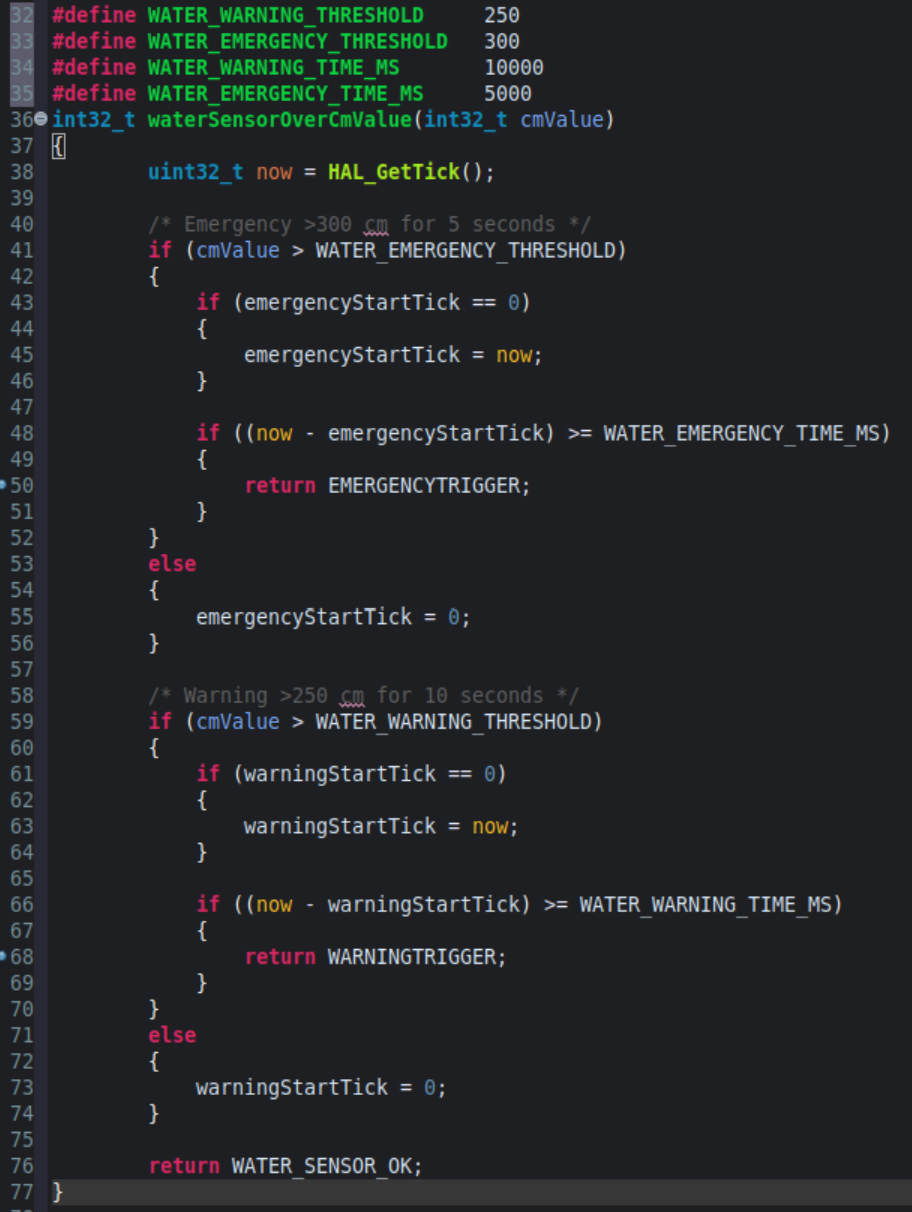
\includegraphics[width=0.75\linewidth]{Pictures/t8.png}
    \caption{Tested code for TC-08}
    \label{fig:t8_code}
\end{figure}
\newpage

%-----------------------------------------------------------------%
    %Test Case 9 - Gas Sensor above Threshold
%-----------------------------------------------------------------%
\section{TC-09 - Gas Sensor above Threshold}

\renewcommand{\arraystretch}{1.4}

\begin{table}[h]
\centering
\begin{tabular}{|p{3cm}|p{12cm}|}
\hline
\textbf{Test Case ID} & TC-09 \\ \hline
\textbf{Description} &  Testing warning and emergency thresholds for gas sensor \\ \hline
\textbf{Prerequisites} & State Operational, gasSensor values are valid and average is calculated \\ \hline
\textbf{Test Steps} &
\begin{enumerate}
\item Loop the 10ms task
\item Manuallyincreasing the ADC values to exceed the defined thresholds
\item Inspect the values in Eclipse
\item Manually modify the ADC values
\item Set a breakpoint on \textit{return EMERGENCYTRIGGER} and \textit{return WARNINGTRIGGER}
\item Verify at which values which breakpoint is triggered
\end{enumerate}
\\ \hline
\textbf{Expected Result} & Breakpoint is triggered \\ \hline
\textbf{Actual Result} & Breakpoint is triggered and for specific values \\ \hline
\textbf{Status} & \textcolor{green!60!black}{Passed} \\ \hline
\end{tabular}
\end{table}
\newpage
\subsection{Description TC-09}
This test case verifies the correct behaviour of the gas sensor monitoring logic when defined
warning and emergency thresholds are exceeded. According to the system requirements, the
application must detect critical gas concentrations and trigger different responses depending
on the severity and duration of the threshold violation.

The function \textit{gasSensorOverPpmValue()} evaluates the averaged gas sensor value and
compares it against the thresholds defined by \textit{GAS\_WARNING\_THRESHOLD} and
\textit{GAS\_EMERGENCY\_THRESHOLD}. If the measured value exceeds 3000\,ppm for at least
5 seconds, the function returns \textit{WARNINGTRIGGER}. If the value exceeds 5000\,ppm
for at least 3 seconds, the function returns \textit{EMERGENCYTRIGGER}.

During the test, the ADC values were manually increased to exceed the specified thresholds.
Breakpoints were placed at the return statements \textit{return WARNINGTRIGGER} and
\textit{return EMERGENCYTRIGGER} in order to verify that the correct trigger is generated
once the respective threshold and time condition are fulfilled.

The successful execution of this test confirms that the system correctly evaluates gas
concentration levels and activates the appropriate warning or emergency condition
according to the specified requirements.
\newpage
\textbf{Tested Code:}

\begin{figure}[h]
    \centering
    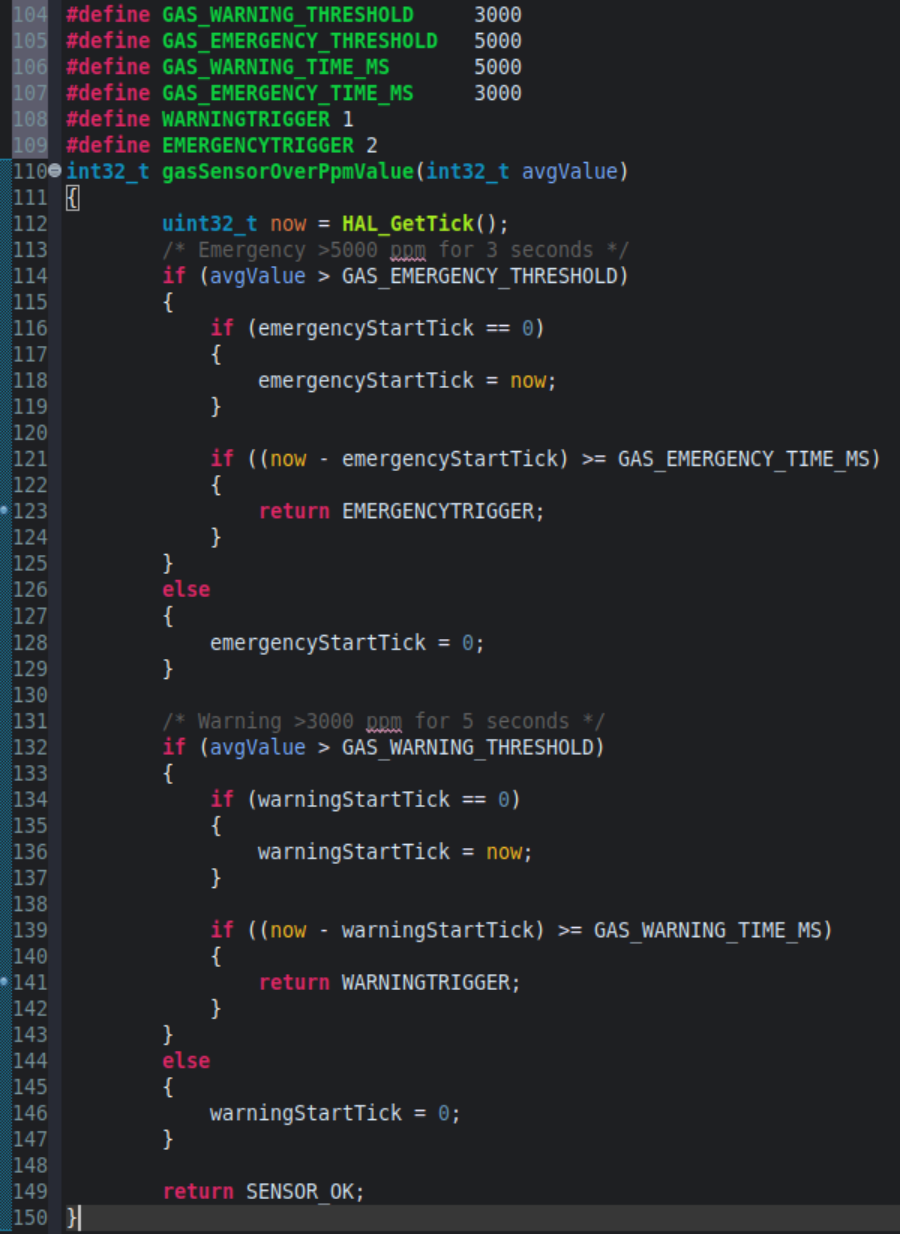
\includegraphics[width=0.75\linewidth]{Pictures/t9.png}
    \caption{Tested code for TC-09}
    \label{fig:t9_code}
\end{figure}
\newpage

%-----------------------------------------------------------------%
    %Test Case 10 - Debouncing Button Presses
%-----------------------------------------------------------------%
\section{TC-10 - Debouncing Button Presses}

\renewcommand{\arraystretch}{1.4}

\begin{table}[h]
\centering
\begin{tabular}{|p{3cm}|p{12cm}|}
\hline
\textbf{Test Case ID} & TC-10 \\ \hline
\textbf{Description} & Verification of the debounce mechanism for push buttons SW1 and B1. \\ \hline
\textbf{Prerequisites} & Operational State, 10ms Task Running \\ \hline
\textbf{Test Steps} &
1. Ensure that both buttons are in released state. \par
2. Press button SW1 quickly several times within a time shorter than the debounce time. \par
3. Observe that no state change event is generated. \par
4. Press button SW1 and hold it longer than the debounce time. \par
5. Verify that the event \textit{APP\_EVT\_SWITCH\_STATE} is triggered. \par
6. Repeat the same procedure with button B1 and verify that event \textit{APP\_EVT\_ALARM\_RESET} is triggered only after the debounce time has passed.
\\ \hline
\textbf{Expected Result} &
Short bouncing signals do not generate any event. A state change event is generated only if the button remains stable for at least the configured debounce time.
\\ \hline
\textbf{Actual Result} & Events are generated only after the debounce time and no false triggers occur during bouncing. \\ \hline
\textbf{Status} & \textcolor{green!60!black}{Passed} \\ \hline
\end{tabular}
\end{table}
\newpage
\subsection{Description TC-10}
This test case verifies the correct functionality of the button debounce mechanism
for the push buttons SW1 and B1. The debounce logic ensures that short mechanical
bouncing signals do not generate unintended events in the application.

The function \textit{debounceButton()} monitors the raw button state and compares it
with the previously recorded state. A state change is only accepted if the signal
remains stable for at least the configured debounce time defined by
\textit{DEBOUNCE\_TIME\_MS}. Once the signal is considered stable, the corresponding
button event is generated by the function \textit{buttonHandler()} via
\textit{applicationSendEvent()}.

For testing purposes, the debounce time was increased from the normal value of
50\,ms to 3 seconds. This made it easier to observe the debounce behaviour during
manual testing and to clearly distinguish between short bouncing signals and a
valid button press.

During the test, the buttons were pressed multiple times within a time shorter
than the debounce period. No events were triggered during these short presses.
Only when the button remained pressed longer than the configured debounce time
did the corresponding events \textit{APP\_EVT\_SWITCH\_STATE} for SW1 or \textit{APP\_EVT\_ALARM\_RESET} for B1 occur.

The successful execution of this test confirms that the debounce mechanism
correctly filters bouncing signals and generates button events only for stable
input signals.
\newpage
\textbf{Tested Code:}

\begin{figure}[h]
    \centering
    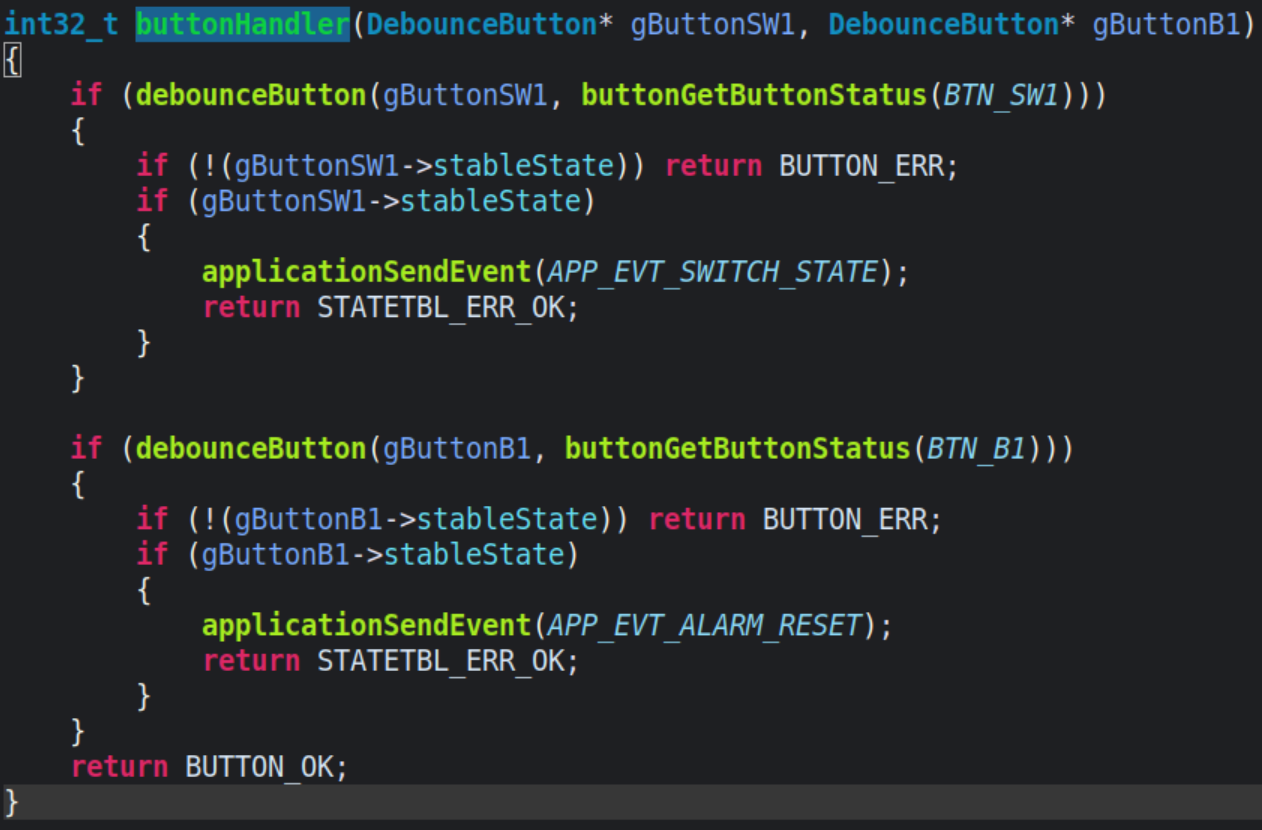
\includegraphics[width=0.75\linewidth]{Pictures/t10_1.png}
    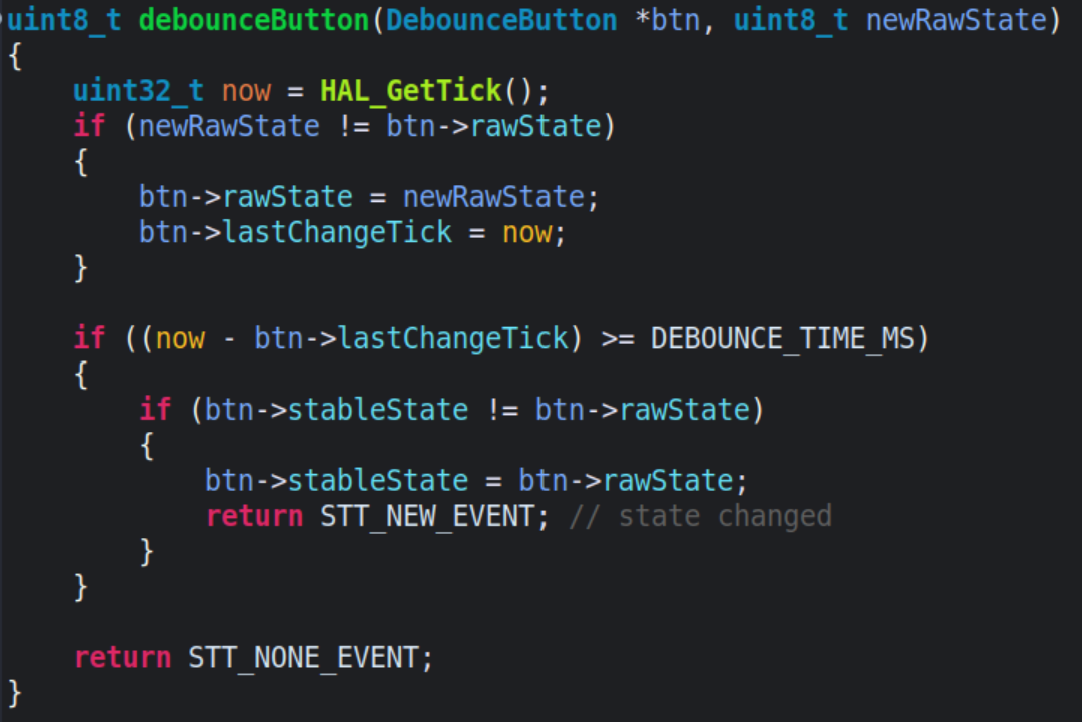
\includegraphics[width=0.75\linewidth]{Pictures/t10_2.png}
    \caption{Tested code for TC-10}
    \label{fig:t10_code}
\end{figure}

\newpage

%-----------------------------------------------------------------%
    %Test Case 11 -
%-----------------------------------------------------------------%
\section{TC-11 - }

\renewcommand{\arraystretch}{1.4}

\begin{table}[h]
\centering
\begin{tabular}{|p{3cm}|p{12cm}|}
\hline
\textbf{Test Case ID} & TC-11 \\ \hline
\textbf{Description} & Testing the transition to the Failure state due to tolerance violation \\ \hline
\textbf{Prerequisites} & State Operational and ADC values are valid \\ \hline
\textbf{Test Steps} &
\begin{enumerate}
\item Execute the 10ms task
\item The constant \textit{PERCENTTOLERANCE} was set to 30 for testing
\item Check the if-condition (see code)
\item Inspect the values in Eclipse
\item Manually modify the ADC values
\item Set a breakpoint on \textit{applicationSendEvent()}
\item Verify at which values the breakpoint is triggered and validate the calculation
\end{enumerate}
\\ \hline
\textbf{Expected Result} & Breakpoint is triggered \\ \hline
\textbf{Actual Result} & Breakpoint is triggered and calculated values match the expected results \\ \hline
\textbf{Status} & \textcolor{green!60!black}{Passed} \\ \hline
\end{tabular}
\end{table}
\newpage
\subsection{Description TC-11}

\textbf{Tested Code:}

\begin{lstlisting}[style=CStyle]
void System_Init(void)
{
    HAL_Init();
    GPIO_Init();
    UART_Init();
}
\end{lstlisting}

\newpage

%-----------------------------------------------------------------%
    %Test Case 12 -
%-----------------------------------------------------------------%
\section{TC-12 - }

\renewcommand{\arraystretch}{1.4}

\begin{table}[h]
\centering
\begin{tabular}{|p{3cm}|p{12cm}|}
\hline
\textbf{Test Case ID} & TC-12 \\ \hline
\textbf{Description} & Testing the transition to the Failure state due to tolerance violation \\ \hline
\textbf{Prerequisites} & State Operational and ADC values are valid \\ \hline
\textbf{Test Steps} &
\begin{enumerate}
\item Execute the 10ms task
\item The constant \textit{PERCENTTOLERANCE} was set to 30 for testing
\item Check the if-condition (see code)
\item Inspect the values in Eclipse
\item Manually modify the ADC values
\item Set a breakpoint on \textit{applicationSendEvent()}
\item Verify at which values the breakpoint is triggered and validate the calculation
\end{enumerate}
\\ \hline
\textbf{Expected Result} & Breakpoint is triggered \\ \hline
\textbf{Actual Result} & Breakpoint is triggered and calculated values match the expected results \\ \hline
\textbf{Status} & \textcolor{green!60!black}{Passed} \\ \hline
\end{tabular}
\end{table}
\newpage
\subsection{Description TC-12}

\textbf{Tested Code:}

\begin{lstlisting}[style=CStyle]
void System_Init(void)
{
    HAL_Init();
    GPIO_Init();
    UART_Init();
}
\end{lstlisting}
